\begin{figure}[htp]
	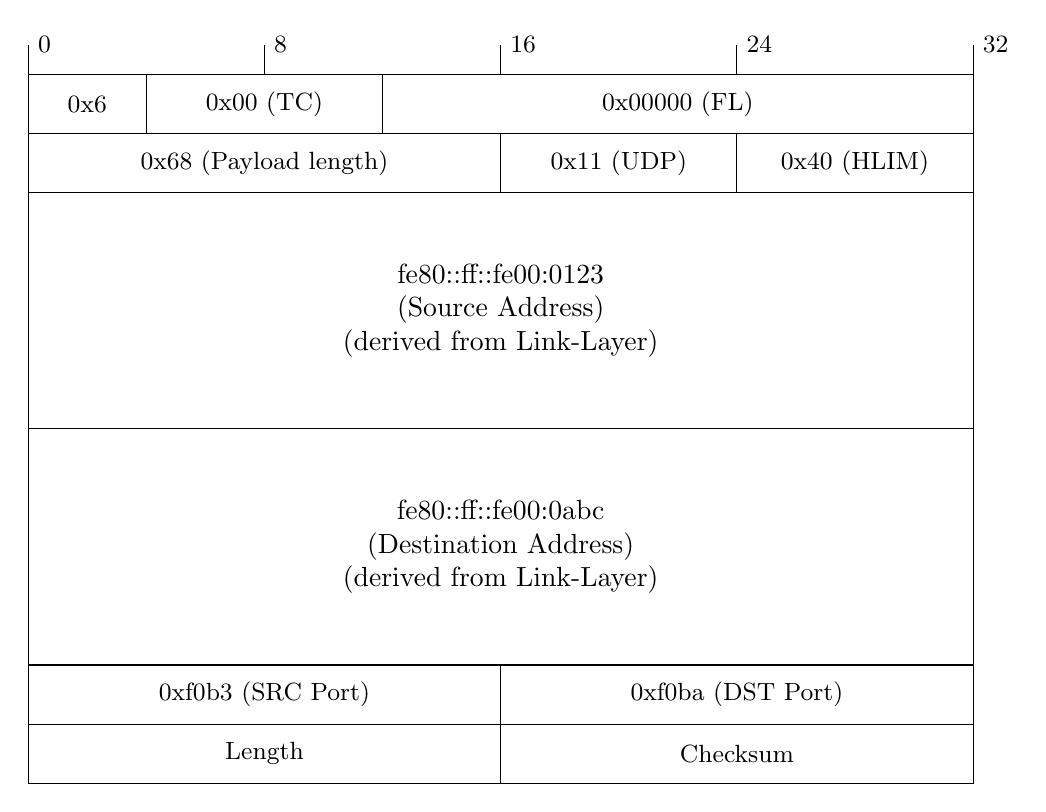
\begin{tikzpicture}[scale=0.75]
		%IPv6
		\draw (0,0) rectangle (16,12);
		\draw (0,11) -- (16,11);
		\draw (0,10) -- (16,10);
		\draw (0,6) -- (16,6);
		\draw (0,2) -- (16,2);
		\draw (0,1) -- (16,1);

		\draw (0,12) -- ++(0,0.5) node[right] {\small 0};
		\draw (4,12) -- ++(0,0.5) node[right] {\small 8};
		\draw (8,12) -- ++(0,0.5) node[right] {\small 16};
		\draw (12,12) -- ++(0,0.5) node[right] {\small 24};
		\draw (16,12) -- ++(0,0.5) node[right] {\small 32};

		\draw (2,12) -- ++(0,-1);
		\node at (1,11.5) {\small 0x6};
		\draw (6,12) -- ++(0,-1);
		\node at (4, 11.5) {\small 0x00 (TC)};
		\node at (11, 11.5) {\small 0x00000 (FL)};

		\draw (8,11) -- ++(0,-1);
		\node at (4, 10.5) {\small 0x68 (Payload length)};
		\draw (12,11) -- ++(0,-1);
		\node at (10, 10.5) {\small 0x11 (UDP)};
		\node at (14,10.5) {\small 0x40 (HLIM)};

		\node at (8, 8) [align=center] {fe80::ff::fe00:0123 \\(Source Address) \\ (derived from Link-Layer)};
		\node at (8, 4) [align=center] {fe80::ff::fe00:0abc \\ (Destination Address) \\ (derived from Link-Layer)};

		\draw (8,2) -- ++(0,-1);
		\node at (4,1.5) {\small 0xf0b3 (SRC Port)};
		\node at (12,1.5) {\small 0xf0ba (DST Port)};

		\draw (8,1) -- ++(0,-1);
		\node at (4,0.5) {\small Length};
		\node at (12,0.5) {\small Checksum};

	\end{tikzpicture}\\
	\vspace{2em}
	48 bytes from the original header result in following 4 bytes:\\
	\vspace{2em}
	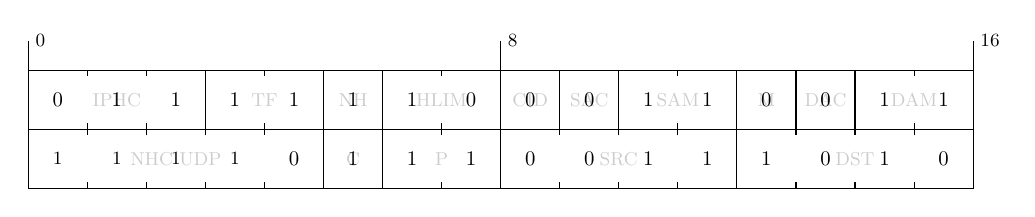
\begin{tikzpicture}[scale=0.75, every node/.append style={scale=0.75}]
		%IPHC
		\draw (0,0) rectangle (16,2);
		\draw (0,1) -- (16,1);
		\draw (0,2) -- ++(0,0.5) node[right] {\small 0};
		\draw (8,2) -- ++(0,0.5) node[right] {\small 8};
		\draw (16,2) -- ++(0,0.5) node[right] {\small 16};

		\foreach \x in {1,2,...,15}{
			\draw (\x,2) -- ++(0,-0.1);
			\draw (\x,1) -- ++(0,0.1);
			\draw (\x,1) -- ++(0,-0.1);
			\draw (\x,0) -- ++(0,0.1);
		}

		\draw (3,1) -- ++(0,1);
		\node at (1.5, 1.5) {\color{black!20}\small IPHC};
		\node at (0.5, 1.5) {0};
		\node at (1.5, 1.5) {1};
		\node at (2.5, 1.5) {1};

		\draw (5,1) -- ++(0,1);
		\node at (4, 1.5) {\color{black!20}\small TF};
		\node at (3.5, 1.5) {1};
		\node at (4.5, 1.5) {1};

		\draw (6,1) -- ++(0,1);
		\node at (5.5, 1.5) {\color{black!20} \small NH};
		\node at (5.5, 1.5) {1};

		\draw (8,1) -- ++(0,1);
		\node at (7, 1.5) {\color{black!20} \small HLIM};
		\node at (6.5, 1.5) {1};
		\node at (7.5, 1.5) {0};

		\draw (9,1) -- ++(0,1);
		\node at (8.5, 1.5) {\color{black!20} \small CID};
		\node at (8.5, 1.5) {0};

		\draw (10,1) -- ++(0,1);
		\node at (9.5, 1.5) {\color{black!20} \small SAC};
		\node at (9.5, 1.5) {0};

		\draw (12,1) -- ++(0,1);
		\node at (11, 1.5) {\color{black!20} \small SAM};
		\node at (10.5, 1.5) {1};
		\node at (11.5, 1.5) {1};

		\draw (13,1) -- ++(0,1);
		\node at (12.5, 1.5) {\color{black!20} \small M};
		\node at (12.5, 1.5) {0};

		\draw (14,1) -- ++(0,1);
		\node at (13.5, 1.5) {\color{black!20} \small DAC};
		\node at (13.5, 1.5) {0};

		\node at (15, 1.5) {\color{black!20} \small DAM};
		\node at (14.5, 1.5) {1};
		\node at (15.5, 1.5) {1};

		%UDP NHC
		\foreach \x in {0.5,1.5,...,3.5}{
			\node at (\x, 0.5) {\small 1};
		}

		\node at (2.5, 0.5) {\color{black!20} \small NHC UDP};

		\node at (4.5, 0.5) {0};
		\draw (5,0) -- ++(0,1);
		\node at (5.5, 0.5) {\color{black!20} \small C};
		\node at (5.5, 0.5) {1};
		\draw (6,0) -- ++(0,1);
		\node at (7, 0.5) {\color{black!20} \small P};
		\node at (6.5, 0.5) {1};
		\node at (7.5, 0.5) {1};
		\draw (8,0) -- ++(0,1);
		\node at (10,0.5) {\color{black!20} \small SRC};
		\node at (8.5, 0.5) {0};
		\node at (9.5, 0.5) {0};
		\node at (10.5, 0.5) {1};
		\node at (11.5, 0.5) {1};
		\draw (12,0) -- ++(0,1);
		\node at (14,0.5) {\color{black!20} \small DST};
		\node at (12.5, 0.5) {1};
		\node at (13.5, 0.5) {0};
		\node at (14.5, 0.5) {1};
		\node at (15.5, 0.5) {0};
		\draw (16,0) -- ++(0,1);
	\end{tikzpicture}
	\caption{Link-Local IPv6 an UDP header to IPHC example}
	\label{fig:6lo_example}
\end{figure}